% generated from JIRA project LVV
% using template at /usr/local/lib/python3.7/site-packages/docsteady/templates/dm-tpr.latex.jinja2.
% using docsteady version 1.2rc24
% Please do not edit -- update information in Jira instead

\documentclass[DM,lsstdraft,STR,toc]{lsstdoc}
\usepackage{geometry}
\usepackage{longtable,booktabs}
\usepackage{enumitem}
\usepackage{arydshln}
\usepackage{attachfile}
\usepackage{array}

\newcolumntype{L}[1]{>{\raggedright\let\newline\\\arraybackslash\hspace{0pt}}p{#1}}

\input meta.tex

\newcommand{\attachmentsUrl}{https://github.com/\gitorg/\lsstDocType-\lsstDocNum/blob/\gitref/attachments}
\providecommand{\tightlist}{
  \setlength{\itemsep}{0pt}\setlength{\parskip}{0pt}}

\setcounter{tocdepth}{4}

\begin{document}

\def\milestoneName{Large Scale CCOB Data Access}
\def\milestoneId{LDM-503-10b}
\def\product{DBB Services}

\setDocCompact{true}

\title{LDM-503-10b: Large Scale CCOB Data Access Test Plan and Report}
\setDocRef{\lsstDocType-\lsstDocNum}
\date{\vcsdate}
\author{ Michelle Butler }

% Most recent last
\setDocChangeRecord{
\addtohist{}{2019-10-22}{Draft}{Michelle Butler}
}

\setDocRef{DMTN-182}
\setDocCurator{Michelle Butler}
\setDocUpstreamLocation{\url{https://github.com/lsst-dm/\lsstDocType-\lsstDocNum}}
\setDocUpstreamVersion{\vcsrevision}



\setDocAbstract{
This is the test plan and report for
\textbf{ Large Scale CCOB Data Access} (LDM-503-10b),
an LSST milestone pertaining to the Data Management Subsystem.
}


\maketitle

\section{Introduction}
\label{sect:intro}


\subsection{Objectives}
\label{sect:objectives}

 Demonstrate the ability to transfer data from the CCOB at SLAC with 21
rafts of data, ~ingest at LDF and make available for viewing and further
processing through an instance of the RSP. ~This is a data transfer of
data from SLAC ~with 21-raft-sized images to NCSA, ingest it into a
Butler environment and place the file into file systems accessible by
the RSP. The CCOB device might NOT be available, but as 21 raft size
data will be available from a test stand at SLAC, we will use a generic
test stand data transfer method (e.g., rsync) to bring designated data
to NCSA, ingest it, and place into appropriate filesystems, and make
available through the RSP. ~This data comes from the Camera Control
System (CCS). ~



\subsection{System Overview}
\label{sect:systemoverview}

 This milestone validates the data from a test stand at SLAC that
contains the test data for 21 rafts single image data with proper
headers. ~ ~That data is to be transferred to the LDF and ingested into
the Butler, and then placed in file systems that are viewable by the
RSP. ~\\[2\baselineskip]

\subsection{Applicable Documents}\label{applicable-documents}

\citeds{LDM-294} Data Management Organization and Management\\
\citeds{LDM-503} DM Test Plan\\
\citeds{LDM-148} Data Management System Design\\
\citeds{LDM-639} Data Management Acceptance Test Specification\\
\citeds{LSE-400} Header Service Interface between the OCS and EFD~


\subsection{Document Overview}
\label{sect:docoverview}

This document was generated from Jira, obtaining the relevant information from the
\href{https://jira.lsstcorp.org/secure/Tests.jspa\#/testPlan/LVV-P55}{LVV-P55}
~Jira Test Plan and related Test Cycles (
\href{https://jira.lsstcorp.org/secure/Tests.jspa\#/testCycle/LVV-C108}{LVV-C108}
).

Section \ref{sect:intro} provides an overview of the test campaign, the system under test (\product{}),
the applicable documentation, and explains how this document is organized.
Section \ref{sect:testplan} provides additional information about the test plan, like for example the configuration
used for this test or related documentation.
Section \ref{sect:personnel} describes the necessary roles and lists the individuals assigned to them.

Section \ref{sect:overview} provides a summary of the test results, including an overview in Table \ref{table:summary},
an overall assessment statement and suggestions for possible improvements.
Section \ref{sect:detailedtestresults} provides detailed results for each step in each test case.

The current status of test plan \href{https://jira.lsstcorp.org/secure/Tests.jspa\#/testPlan/LVV-P55}{LVV-P55} in Jira is \textbf{ Completed }.

\subsection{References}
\label{sect:references}
\renewcommand{\refname}{}
\bibliography{lsst,refs,books,refs_ads,local}


\newpage
\section{Test Plan Details}
\label{sect:testplan}


\subsection{Data Collection}

  Observing is not required for this test campaign.

\subsection{Verification Environment}
\label{sect:hwconf}

  \subsection{Entry Criteria}
  Images taken and sent to NCSA through CCS data transfer mechanisms.~
~\\[2\baselineskip]

  \subsection{Exit Criteria}
  Data is viewable on RSP which means that it was ingested and placed in a
Butler repo. ~


\subsection{Related Documentation}


No additional documentation provided.


\subsection{PMCS Activity}

Primavera milestones related to the test campaign:
\begin{itemize}
\item LDM-503-10b
\end{itemize}


\newpage
\section{Personnel}
\label{sect:personnel}

The personnel involved in the test campaign is shown in the following table.

{\small
\begin{longtable}{p{3cm}p{3cm}p{3cm}p{6cm}}
\hline
\multicolumn{2}{r}{T. Plan \href{https://jira.lsstcorp.org/secure/Tests.jspa\#/testPlan/LVV-P55}{LVV-P55} owner:} &
\multicolumn{2}{l}{\textbf{ Michelle Butler } }\\\hline
\multicolumn{2}{r}{T. Cycle \href{https://jira.lsstcorp.org/secure/Tests.jspa\#/testCycle/LVV-C108}{LVV-C108} owner:} &
\multicolumn{2}{l}{\textbf{
Michelle Butler }
} \\\hline
\textbf{Test Cases} & \textbf{Assigned to} & \textbf{Executed by} & \textbf{Additional Test Personnel} \\ \hline
\href{https://jira.lsstcorp.org/secure/Tests.jspa#/testCase/LVV-T1556}{LVV-T1556}
& {\small Michelle Butler } & {\small Michelle Butler } &
\begin{minipage}[]{6cm}
\smallskip
{\small  }
\medskip
\end{minipage}
\\ \hline
\end{longtable}
}

\newpage

\section{Test Campaign Overview}
\label{sect:overview}

\subsection{Summary}
\label{sect:summarytable}

{\small
\begin{longtable}{p{2cm}cp{2.3cm}p{8.6cm}p{2.3cm}}
\toprule
\multicolumn{2}{r}{ T. Plan \href{https://jira.lsstcorp.org/secure/Tests.jspa\#/testPlan/LVV-P55}{LVV-P55}:} &
\multicolumn{2}{p{10.9cm}}{\textbf{ LDM-503-10b: Large Scale CCOB Data Access }} & Completed \\\hline
\multicolumn{2}{r}{ T. Cycle \href{https://jira.lsstcorp.org/secure/Tests.jspa\#/testCycle/LVV-C108}{LVV-C108}:} &
\multicolumn{2}{p{10.9cm}}{\textbf{ LDM-503-10b Large Scale CCOB Data Access }} & Done \\\hline
\textbf{Test Cases} &  \textbf{Ver.} & \textbf{Status} & \textbf{Comment} & \textbf{Issues} \\\toprule
\href{https://jira.lsstcorp.org/secure/Tests.jspa#/testCase/LVV-T1556}{LVV-T1556}
&  1
& Pass &
\begin{minipage}[]{9cm}
\smallskip
Data transferred (20090 files) to NCSA on 8/19/2020. ~The files were
transferred to NCSA and were ingested into the directory(20086 files; 4
were zero length):
/lsstdata/offline/teststand/BOT/storage/20200819\\[2\baselineskip]
\medskip
\end{minipage}
&   \\\hline
\caption{Test Campaign Summary}
\label{table:summary}
\end{longtable}
}

\subsection{Overall Assessment}
\label{sect:overallassessment}

CCOB (camera control system) CCS images were transferred to NCSA through
the rsync utilitiy (CCS method of data transfer) . ~ Data was ingested
by cron job at NCSA into a Gen2 repo and was made available on the RSP
for further review and processing by scientific staff. ~ Here is a
notebook that allows the image generation from the 21 raft data: ~
github:
~https://github.com/lsst-dm/\citeds{DMTR-182}/tree/executions/pinholes.ipynb\\
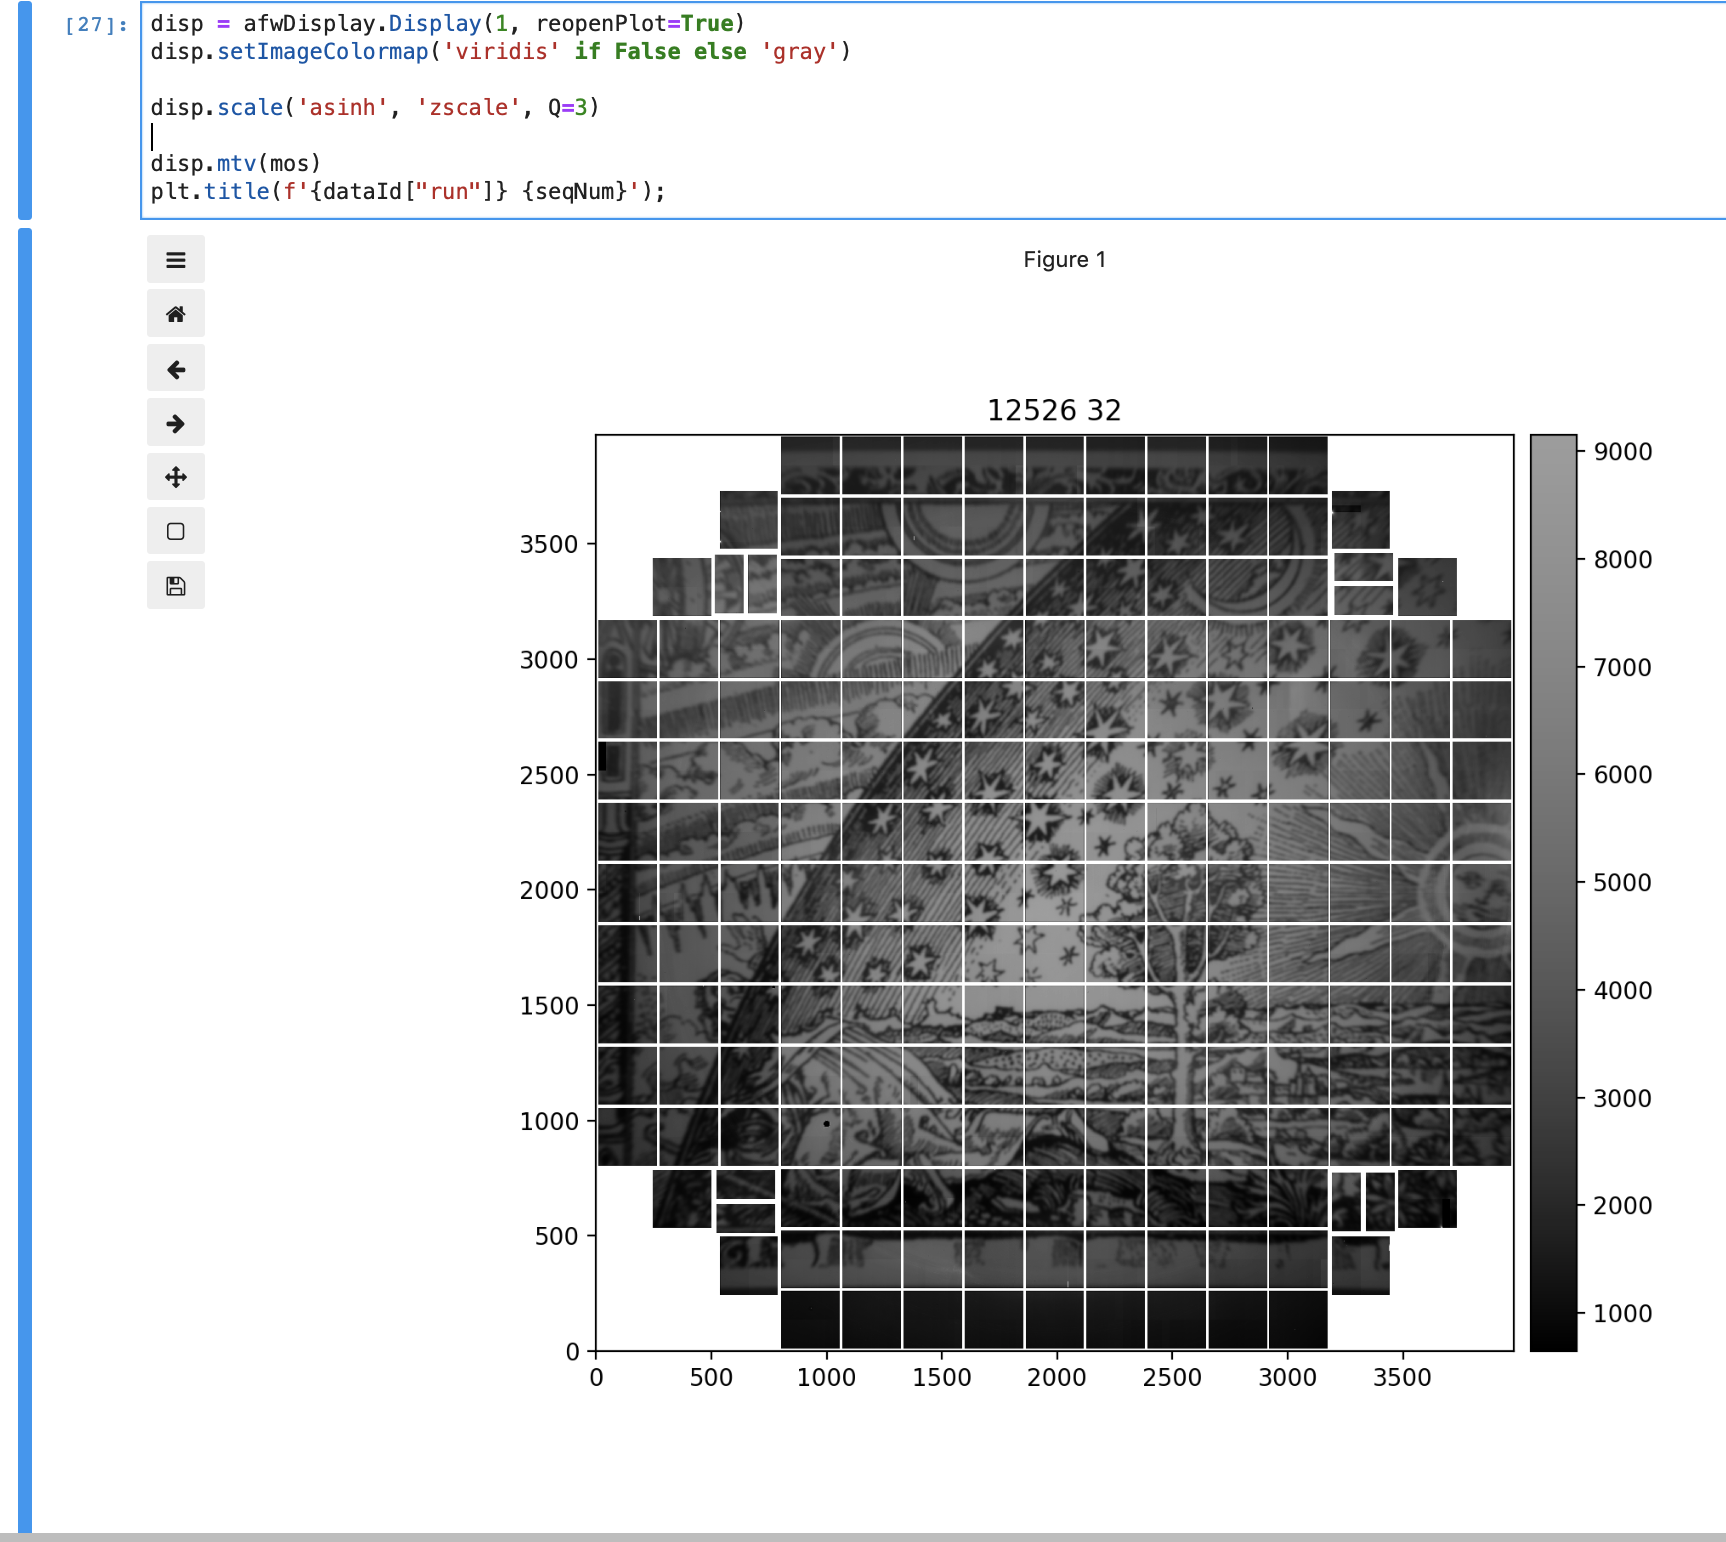
\includegraphics[width=3.12500in]{jira_imgs/1550.png}

\subsection{Recommended Improvements}
\label{sect:recommendations}

The current data transfer method is too slow for quick changes to the
camera and images as the CCOB is currently at SLAC. ~The timing will
change once the CCOB is placed on the mountain. ~This is temporary due
to the environment at SLAC. ~ NCSA then ingests the data into a butler
repo as the file arrives at NCSA. ~ ~ ~ A suggestion of the RSP be
installed at SLAC so that images can be retrieved quickly and changes to
the camera could be quicker. ~ The data at SLAC must be moved to a node
that is accessible to ~an outside internet connection which is able to
reach NCSA. ~This has taken in the past hours. ~ The data is then
``rsynced'' to NCSA. ~ ~ Currently after the files are placed in a
outside visible node, each file takes on average 4 seconds to be
transferred and ingested. ~ ~Depending on how long the CCS environment
stays at SLAC, will put priority on how much effort needs to go into
making these transfer mechanisms faster or not. ~ ~\\[2\baselineskip]As
the CCOB for 21 RAFT data moves from SLAC to the mountain, the CCS data
will be available immediately to be transferred to NCSA or available on
the telemetry cluster that can have a RSP environment installed for
immediate viewing. This. slowness of the CCOB data is temporary due to
it's location at SLAC.~~\\[2\baselineskip]

\newpage
\section{Detailed Test Results}
\label{sect:detailedtestresults}

\subsection{Test Cycle LVV-C108 }

Open test cycle {\it \href{https://jira.lsstcorp.org/secure/Tests.jspa#/testrun/LVV-C108}{LDM-503-10b Large Scale CCOB Data Access}} in Jira.

Test Cycle name: LDM-503-10b Large Scale CCOB Data Access\\
Status: Done

Demonstrate the ability to transfer data from the CCOB with 21 rafts
from SLAC and ingested at NCSA and make available through an instance of
the RSP (Rubin Science Platform)\\[2\baselineskip]

\subsubsection{Software Version/Baseline}
Not provided.

\subsubsection{Configuration}
The data at SLAC is 21 rafts of 9CCD image with proper headers at SLAC.
~ The data transfer environment installed on SLAC systems for specific
diretories only. ~Data transfer environment at NCSA. ~Ingest software
installed at LDF. ~RSP environment installed at NCSA. ~~

\subsubsection{Test Cases in LVV-C108 Test Cycle}

\paragraph{ LVV-T1556 - LDM-503-10B Large Scale CCOB Data Access }\mbox{}\\

Version \textbf{1}.
Open  \href{https://jira.lsstcorp.org/secure/Tests.jspa#/testCase/LVV-T1556}{\textit{ LVV-T1556 } }
test case in Jira.

Demonstrate the ability to transfer data from the SLAC test stand or
CCOB with 21 rafts from SLAC and ingested at NCSA and make available
through an instance of the RSP

\textbf{ Preconditions}:\\
SLAC or some other test stand needs to have produced 21 rafts of data
that has some environment for transferring the data to NCSA. ~ ~The
images won't be able to be ingested at NCSA into butler repositories if
the headers are not correct. ~ ~The \citeds{LSE-400} document calls out what
fields are designed to be completed by the image properly.~ ~The headers
at this time are still in test form, and are being updated as images are
created.~ ~ The confluence page
of:~\url{https://confluence.lsstcorp.org/display/SYSENG/ComCam+Header+Information+Topic+Mapping}
has the current header configuration and what the information maps to
for the ingest information.~ ~

Execution status: {\bf Pass }

Final comment:\\Data transferred (20090 files) to NCSA on 8/19/2020. ~The files were
transferred to NCSA and were ingested into the directory(20086 files; 4
were zero length):
/lsstdata/offline/teststand/BOT/storage/20200819\\[2\baselineskip]


Detailed steps results:

\begin{longtable}{p{1cm}p{15cm}}
\hline
{Step} & Step Details\\ \hline
1 & Description \\
 & \begin{minipage}[t]{15cm}
{\footnotesize
Have a system at SLAC that has the 21 raft data that needs to be
transferred to NCSA, and all accounts and scripts installed on
environment that can read that data.~ ~

\medskip }
\end{minipage}
\\ \cdashline{2-2}

 & Test Data \\
 & \begin{minipage}[t]{15cm}{\footnotesize
21 rafts of data with proper headers~

\medskip }
\end{minipage} \\ \cdashline{2-2}

 & Expected Result \\
 & \begin{minipage}[t]{15cm}{\footnotesize
scripts are able to transfer the data to NCSA though rsync or bbcp.
~\\[2\baselineskip]

\medskip }
\end{minipage} \\ \cdashline{2-2}

 & Actual Result \\
 & \begin{minipage}[t]{15cm}{\footnotesize
SLAC started in late August with the main telescope camera (MTCam)
having the ability to generate 21 raft scale images. ~\\[2\baselineskip]

\medskip }
\end{minipage} \\ \cdashline{2-2}

 & Status: \textbf{ Pass } \\ \hline

2 & Description \\
 & \begin{minipage}[t]{15cm}
{\footnotesize
Data is transferred to NCSA and ingested into Butler~

\medskip }
\end{minipage}
\\ \cdashline{2-2}

 & Test Data \\
 & \begin{minipage}[t]{15cm}{\footnotesize
21 rafts of data~

\medskip }
\end{minipage} \\ \cdashline{2-2}

 & Expected Result \\
 & \begin{minipage}[t]{15cm}{\footnotesize
Data is transferred to NCSA, and can now be see in file systems by the
RSP. ~\\[2\baselineskip]

\medskip }
\end{minipage} \\ \cdashline{2-2}

 & Actual Result \\
 & \begin{minipage}[t]{15cm}{\footnotesize
Data was transferred and ingested into Gen2
Butler:~/lsstdata/offline/teststand/BOT/storage/20200819

\medskip }
\end{minipage} \\ \cdashline{2-2}

 & Status: \textbf{ Pass } \\ \hline

3 & Description \\
 & \begin{minipage}[t]{15cm}
{\footnotesize
using the RSP view the data in the ingested directory~

\medskip }
\end{minipage}
\\ \cdashline{2-2}

 & Test Data \\
 & \begin{minipage}[t]{15cm}{\footnotesize
21 rafts of data with proper headers and available with Butler.get~

\medskip }
\end{minipage} \\ \cdashline{2-2}

 & Expected Result \\
 & \begin{minipage}[t]{15cm}{\footnotesize
data can be viewed.

\medskip }
\end{minipage} \\ \cdashline{2-2}

 & Actual Result \\
 & \begin{minipage}[t]{15cm}{\footnotesize
Data is available on the RSP:
/lsstdata/offline/teststand/BOT/storage/20200819\\[2\baselineskip]

\medskip }
\end{minipage} \\ \cdashline{2-2}

 & Status: \textbf{ Pass } \\ \hline

\end{longtable}


\newpage
\appendix

\section{Traceability}

\begin{longtable}{p{3cm}p{3cm}L{9cm}}
\hline
\textbf{Test Case} & \textbf{VE Key} & \textbf{VE Summary} \\ \hline
\href{https://jira.lsstcorp.org/secure/Tests.jspa#/testCase/LVV-T1556}{LVV-T1556} &
  \href{https://jira.lsstcorp.org/browse/LVV-8}{LVV-8}
  & DMS-REQ-0018-V-01: Raw Science Image Data Acquisition
 \\ \cdashline{2-3}
 &   \href{https://jira.lsstcorp.org/browse/LVV-9}{LVV-9}
  & DMS-REQ-0020-V-01: Wavefront Sensor Data Acquisition
 \\ \cdashline{2-3}
 &   \href{https://jira.lsstcorp.org/browse/LVV-11}{LVV-11}
  & DMS-REQ-0024-V-01: Raw Image Assembly
 \\ \cdashline{2-3}
 &   \href{https://jira.lsstcorp.org/browse/LVV-146}{LVV-146}
  & DMS-REQ-0315-V-01: DMS Communication with OCS
 \\ \cdashline{2-3}
 &   \href{https://jira.lsstcorp.org/browse/LVV-28}{LVV-28}
  & DMS-REQ-0068-V-01: Raw Science Image Metadata
 \\ \cdashline{2-3}
\hline
\end{longtable}


\newpage
%Make sure lsst-texmf/bin/generateAcronyms.py is in your path
\section{Acronyms used in this document}\label{sec:acronyms}
\addtocounter{table}{-1}
\begin{longtable}{p{0.145\textwidth}p{0.8\textwidth}}\hline
\textbf{Acronym} & \textbf{Description}  \\\hline

CCOB & Camera Calibration Optical Bench \\\hline
DM & Data Management \\\hline
DMTN & DM Technical Note \\\hline
LDF & LSST Data Facility \\\hline
LDM & LSST Data Management (Document Handle) \\\hline
LSP & LSST Science Platform \\\hline
LSST & Large Synoptic Survey Telescope \\\hline
NCSA & National Center for Supercomputing Applications \\\hline
SLAC & SLAC National Accelerator Laboratory (formerly Stanford Linear Accelereator Center; SLAC is now no longer an acronym) \\\hline
\end{longtable}


\end{document}
